
{\tiny

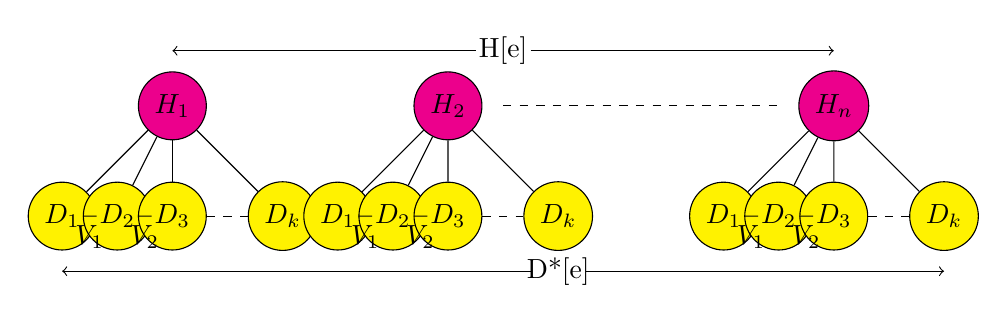
\begin{tikzpicture}[scale=0.7, every node/.style={minimum size=5pt}]

% Define the central nodes
\node[draw, circle, fill=magenta, minimum size=5pt] (H1) at (0, 2) {$H_1$};
\node[draw, circle, fill=yellow] (node1_1) at (-2, 0) {$D_1$};
\node[draw, circle, fill=yellow] (node2_1) at (-1, 0) {$D_2$};
\node[draw, circle, fill=yellow] (node3_1) at (0, 0) {$D_3$};
% \node[draw, circle, fill=yellow] (node4_1) at (1.5, 0) {$D_{k-1}$};
\node[draw, circle, fill=yellow] (node5_1) at (2, 0) {$D_k$};
\draw (H1) -- (node1_1) -- node[midway, below] {$V_1$} (node2_1);
\draw (H1) -- (node2_1) -- node[midway, below] {$V_2$} (node3_1);
\draw (H1) -- (node3_1) ;
\draw[dashed] (node3_1) -- (node5_1);
% \draw (H1) -- (node4_1) -- node[midway, below] {$V_{k-1}$} (node5_1);
\draw (H1) -- (node5_1);

% Second star network (shifted by 12 units to the right)
\node[draw, circle, fill=magenta, minimum size=5pt] (H2) at (5, 2) {$H_2$};
\node[draw, circle, fill=yellow] (node1_2) at (3, 0) {$D_1$};
\node[draw, circle, fill=yellow] (node2_2) at (4, 0) {$D_2$};
\node[draw, circle, fill=yellow] (node3_2) at (5, 0) {$D_3$};
% \node[draw, circle, fill=yellow] (node4_2) at (7.5, 0) {$D_{k-1}$};
\node[draw, circle, fill=yellow] (node5_2) at (7, 0) {$D_k$};
\draw (H2) -- (node1_2) -- node[midway, below] {$V_1$} (node2_2);
\draw (H2) -- (node2_2) -- node[midway, below] {$V_2$} (node3_2);
\draw (H2) -- (node3_2);
\draw[dashed] (node3_2) -- (node5_2);
% \draw (H2) -- (node4_2) -- node[midway, below] {$V_{k-1}$} (node5_2);
\draw (H2) -- (node5_2);

% Third star network (shifted by 24 units to the right)
\node[draw, circle, fill=magenta, minimum size=5pt] (H3) at (12, 2) {$H_n$};
\node[draw, circle, fill=yellow] (node1_3) at (10, 0) {$D_1$};
\node[draw, circle, fill=yellow] (node2_3) at (11, 0) {$D_2$};
\node[draw, circle, fill=yellow] (node3_3) at (12, 0) {$D_3$};
% \node[draw, circle, fill=yellow] (node4_3) at (13.5, 0) {$D_{k-1}$};
\node[draw, circle, fill=yellow] (node5_3) at (14, 0) {$D_k$};
\draw (H3) -- (node1_3) -- node[midway, below] {$V_1$} (node2_3);
\draw (H3) -- (node2_3) -- node[midway, below] {$V_2$} (node3_3);
\draw (H3) -- (node3_3) ;
\draw[dashed] (node3_3) -- (node5_3);
% \draw (H3) -- (node4_3) -- node[midway, below] {$V_{k-1}$} (node5_3);
\draw (H3) -- (node5_3);

\draw [dashed] (6,2) -- (11,2);

\draw [->, ] (6.5,-1) -- (-2,-1);

\draw [->, ] (7.5,-1) -- (14,-1);

\node at (7,-1){D*[e]};

\draw [->, ] (5.5,3) -- (0,3);

\draw [->, ] (6.5,3) -- (12,3);

\node at (6,3){H[e]};


\end{tikzpicture}

}
